\fancyhead{}
\fancyfoot{}
\newtheorem{teorema}{Teorema}
\cfoot{\thepage}


\lhead{Conceptos fundamentales, teorías y antecedentes}
%\rhead{\today}
%\rfoot{\thepage}

\chapter{Conceptos fundamentales, teorías y antecedentes}
Este capítulo tiene como finalidad presentar los conceptos teóricos esenciales y los antecedentes más relevantes que enmarcan el desarrollo del "Sistema de Asistencia Basado en Reconocimiento Facial para la FPUNE". En primer lugar, se abordan las ideas fundamentales relacionadas con la biometría, la inteligencia artificial, y el reconocimiento facial, permitiendo así comprender las bases científicas y técnicas sobre las que se construye esta propuesta.
Posteriormente, se incluyen trabajos previos desarrollados por otros autores, tanto a nivel local como internacional, que sirvieron de referencia y aportaron enfoques valiosos al diseño de la presente solución. Dichos antecedentes permiten contextualizar el problema, identificar soluciones existentes, evaluar sus resultados y reconocer las oportunidades de mejora que esta investigación busca abordar.
\section{Conceptos fundamentales}
\subsection{Historia de la biometría}
La biometría no se puso en práctica en las culturas occidentales hasta f
inales del siglo XIX, pero era utilizada en China desde al menos el siglo XIV.
Un explorador y escritor que responía al nombre de Joao de Barros escribió
que los comerciantes chinos estampaban las impresiones y las huellas de la
palma de las manos de los niños en papel con tinta. Los comerciantes hacían
esto como método para distinguir entre los niños jóvenes.

En Occidente, la identificación confiaba simplemente en la "memoria fotográfica” hasta que Alphonse Bertillon, jefe del departamento fotográfico de
la Policía de París, desarrolló el sistema antropométrico (también conocido
más tarde como Bertillonage) en 1883. Este era el primer sistema preciso, ampliamente utilizado científicamente para identificar a criminales y convirtió a
la biométrica en un campo de estudio.

Funcionaba midiendo de forma precisa ciertas longitudes y anchuras de la
cabeza y del cuerpo, Así como registrando marcas individuales como tatuajes
y cicatrices. El sistema de Bertillon fue adoptado extensamente en occidente
hasta que aparecieron defectos en el sistema, principalmente problemas con
métodos distintos de medidas y cambios de medida. Después de esto, las fuerzas
policiales occidentales comenzaron a usar la huella dactilar esencialmente el
mismo sistema visto en China cientos de años antes[5].


\subsection{Concepto de Seguridad Biométrica}

Para abordar el concepto de seguridad biométrica, es fundamental primero comprender qué es la biometría. Es la ciencia del análisis de las características
físicas o del comportamiento, propias de cada individuo, con el fin de autenticar su identidad. En el sentido literal y el más simple, la biometría significa la
"medición del cuerpo humano"[6].

La biometría es la medición estadística y matemática de características
físicas o biológicas únicas con fines de identificación[7].


Los datos biométricos son cualquier tipo de información sobre las características físicas de un individuo, como los patrones de la retina, las huellas
dactilares y la estructura facial [7].



\begin{figure}[H]
  \centering
  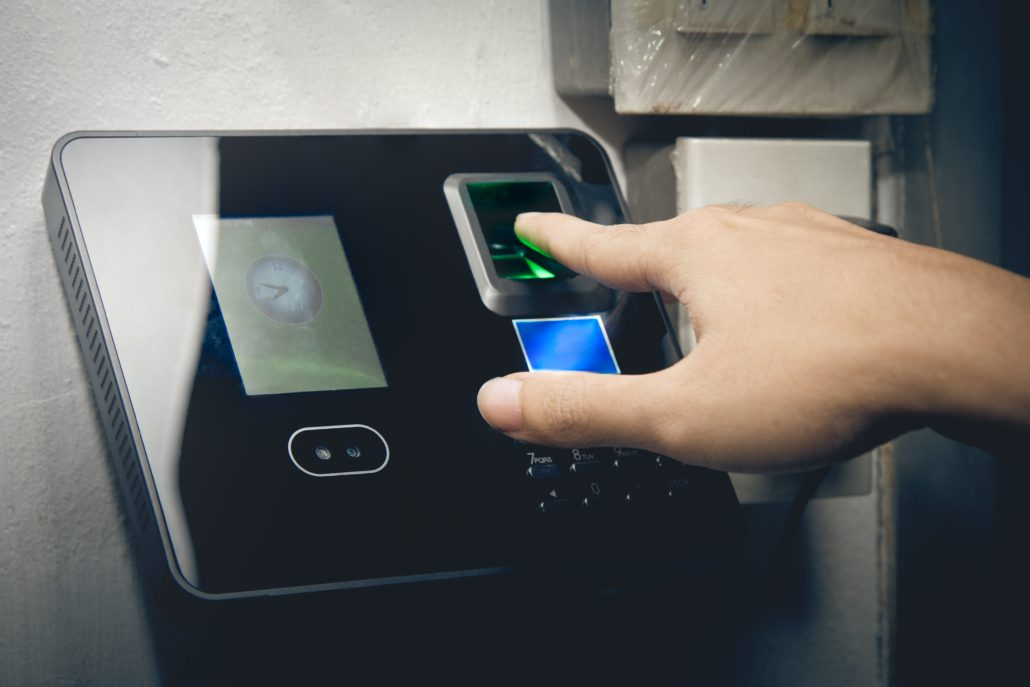
\includegraphics[width=0.6\textwidth]{imagenes_doc/segu_biometrica_1.jpg}
  \caption{Ejemplo de Seguridad Biométrica}
  \label{fig:logo}
\end{figure}

La seguridad biométrica se refiere al uso de características biológicas únicas para la autenticación digital y control de acceso. Los componentes de
hardware, como las cámaras o los lectores de huellas dactilares, recogen los
datos biométricos, que se escanean y se comparan algorítmicamente con la
información contenida en una base de datos. Si los dos conjuntos de datos
coinciden, se autentica la identidad y se concede el acceso [7].



\subsection{Historia de Reconocimiento Facial}


En 1960, Woodrow Wilson Bledsoe trabajó en un sistema para clasificar los
rasgos del rostro humano a través de la tabla RAND. Este sistema utilizaba
un lápiz óptico y unas coordenadas para situar los ojos, la nariz o la boca de las
personas de forma precisa, pero era un procedimiento todavía muy manual [1].

\begin{figure}[H]
  \centering
  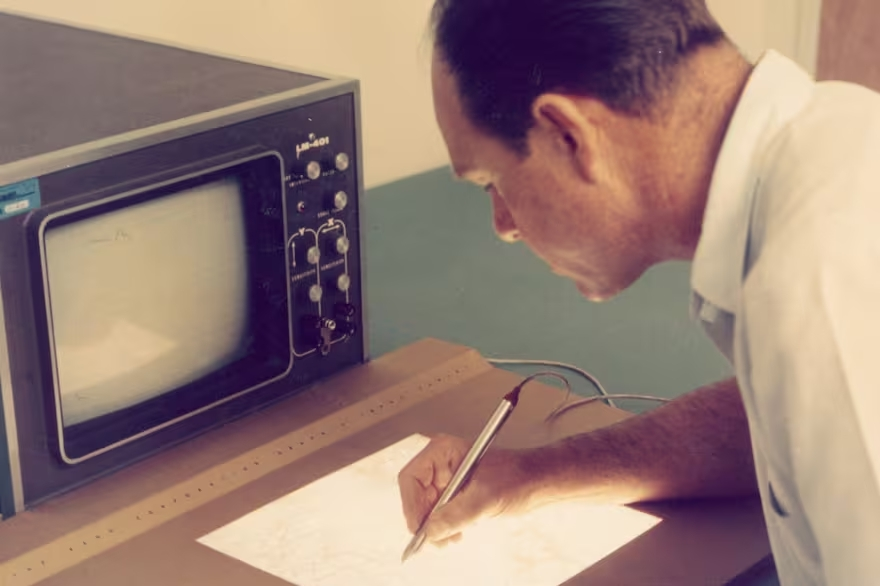
\includegraphics[width=0.6\textwidth]{imagenes_doc/tabla_rand.jpg}
  \caption{Una vista de la tableta digitalizadora de RAND; creada en la década de 1960, en la que se probó el primer sistema de identificación facial}
  \label{fig:logo}
\end{figure}



Una década después llegarían Goldstein, Harmon y Lesk, que detallaron
estas características faciales e iniciaron la mejora hacia la precisión del reconocimiento facial. Más adelante, a finales de los años 80', se aplica el
álgebra lineal, gracias a Sirovich y Kirby.


Ya en 1991, Turk y Pentland desarrollan la tecnología capaz de detectar
un rostro humano dentro de una fotografía, abriendo paso al reconoci
miento facial automático.


Poco a poco, el reconocimiento facial se fue haciendo un hueco en las aplicaciones de seguridad, en particular aquellas concernientes al Estado. En
2001, nace el Viola-Jones Object Detection Framework, que propone algoritmos para detectar objetos dentro de imágenes, y que enseguida fue utilizado
para la detección de rostros de forma exitosa. No es hasta 2010 cuando esta
tecnología llega al gran público a través de Facebook [1].


\subsection{Concepto del Reconocimiento Facial}

El reconocimiento facial es una manera de identificar o confirmar la identi
dad de una persona mediante su rostro. Los sistemas de reconocimiento facial
se pueden utilizar para identificar a las personas en fotos, videos o en tiempo
real.

\begin{figure}[H]
  \centering
  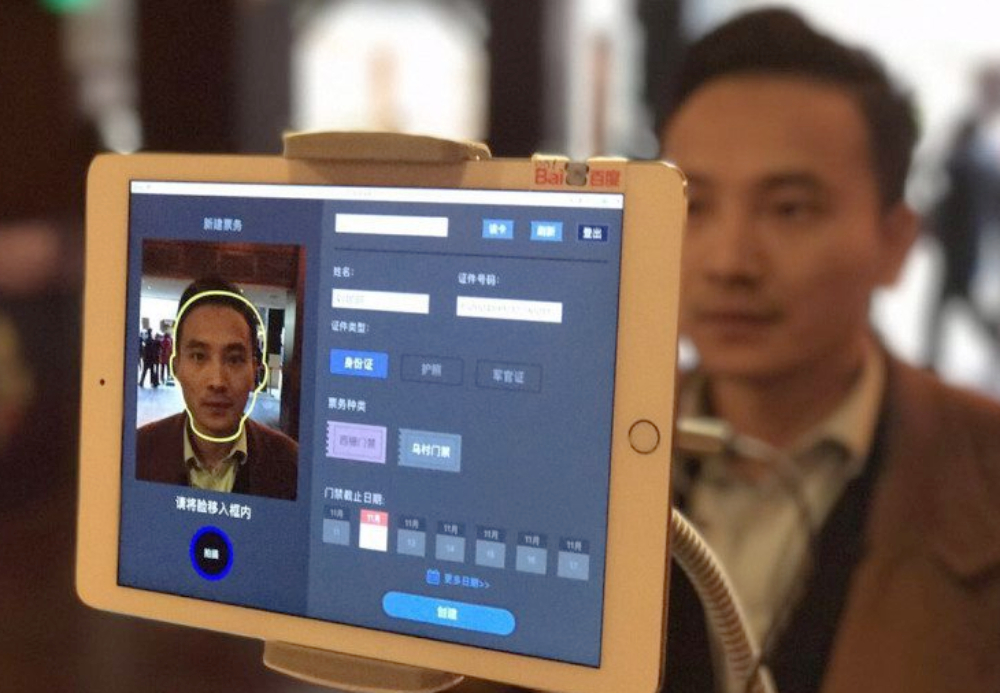
\includegraphics[width=0.6\textwidth]{imagenes_doc/Reconocimiento_Facial.jpg}
  \caption{Dispositivo de reconocimiento facial utilizado en un aeropuerto para verificar la identidad de los pasajeros mediante el análisis de sus rasgos faciales en tiempo real.}
  \label{fig:logo}
\end{figure}



El reconocimiento facial es una categoría de seguridad biométrica. Otras
formas de software biométrico incluyen el reconocimiento de voz, el reconoci
miento de huellas digitales y el reconocimiento de retina o iris. La tecnología
se utiliza principalmente para la protección y las fuerzas de seguridad, aunque
hay un creciente interés en otras áreas de uso [8].


\subsection{Funcionamiento del Reconocimiento Facial}

\begin{itemize}
  \item \textbf{Paso 1: Reconocimiento Facial} 
La cámara detecta y ubica la imagen de un rostro, ya sea de forma independiente o como parte de una muchedumbre. La imagen puede mostrar a la
persona de frente o de perfil.
  \item \textbf{Paso 2: Análisis facial}
A continuación, se captura y analiza una imagen del rostro. La mayor parte
de la tecnología de reconocimiento facial depende de imágenes 2D en lugar de
3D, ya que se puede comparar de manera más fácil una imagen 2D con las
fotos públicas o las de una base de datos. El software lee la geometría de tu
rostro. Los factores clave incluyen la distancia entre los ojos, la profundidad de
las cuencas de los ojos, la distancia desde la frente hasta el mentón, la forma
de los pómulos y el contorno de los labios, las orejas y el mentón El objetivo
es identificar los puntos de referencia faciales que son clave para distinguir un
rostro.
  \item \textbf{Paso 3: Conversión de la imagen a datos}
El proceso de captura de rostro transforma la información analógica (un
rostro) en un conjunto de información digital (datos) basado en los rasgos faciales de la persona. Básicamente, el análisis del rostro se convierte en una
fórmula matemática. El código numérico se denomina huella facial. De la mis
ma manera en que las huellas dactilares son únicas, cada persona tiene su
propia huella facial.
  \item \textbf{Paso 4: Búsqueda de una coincidencia}
La huella facial se compara con una base de datos de otros rostros conocidos. Por ejemplo, el FBI tiene acceso a hasta 650 millones de fotos, de diversas
bases de datos estatales. Si la huella facial coincide con una imagen en una base
de datos de reconocimiento facial, entonces se realizará una determinación.

De todas las mediciones biométricas, el reconocimiento facial se considera
el más natural. Esto sigue una lógica intuitiva, ya que normalmente nos reconocemos a nosotros mismos y a los dem´ as mirando las caras, en lugar de
las huellas digitales y los iris. Se estima que, periódicamente, más de la mitad
de la población mundial se ve afectada por la tecnología de reconocimiento
facial [8].
\end{itemize}


\subsection{Aplicaciones de los sistemas de reconocimiento facial.}
Para abordar el tema de las aplicaciones de los sistemas de reconocimiento
facial, se explorarán tres áreas clave:


\begin{itemize}
  \item \textbf{Detección de fraudes:} Las empresas utilizan el reconocimiento facial para identificar de forma
exclusiva a los usuarios que crean una nueva cuenta en una plataforma en
línea. Una vez que esto se realiza, se puede utilizar el reconocimiento facial
para verificar la identidad de la persona que realmente utiliza la cuenta en
caso de que se produzca una actividad de riesgo o sospechosa en la cuenta.
  \item \textbf{Seguridad cibernética:}Las empresas utilizan la tecnología de reconocimiento facial en lugar de
las contraseñas para reforzar las medidas de seguridad cibernética. Es difícil
acceder sin autorización a los sistemas de reconocimiento facial, ya que no se
puede cambiar nada del rostro. El software de reconocimiento facial también
es una herramienta de seguridad cómoda y de gran precisión para desbloquear
teléfonos inteligentes y otros dispositivos personales.
  \item \textbf{Control de aeropuertos y fronteras:} Muchos aeropuertos utilizan los datos biométricos como pasaportes, con lo
que los viajeros pueden evitar las largas filas y pasar por una terminal automatizada para llegar más rápidamente a la puerta de embarque. La tecnología de
reconocimiento facial en forma de pasaportes electrónicos reduce los tiempos de espera y mejora la seguridad [3].
\end{itemize}


\subsection{Precisión del Reconocimiento Facial}

Los algoritmos de reconocimiento facial tienen una precisión casi perfecta
en condiciones ideales. Existe una mayor tasa de éxito en entornos controlados,
pero generalmente una tasa de rendimiento inferior en el mundo real. Es difícil
predecir con exactitud la tasa de éxito de esta tecnología, ya que ninguna
medida única proporciona un panorama completo.


Por ejemplo, los algoritmos de verificación facial que buscan coincidencias
entre personas e imágenes de referencia claras, como una licencia de conducción
o una foto policial, logran puntuaciones de alta precisión. Sin embargo, este
nivel de precisión únicamente es posible con lo siguiente:


\begin{itemize}
  \item Posicionamiento e iluminación coherentes
  \item Rasgos faciales claros y libres de obstrucciones
  \item Colores y fondo controlados
  \item Calidad de la cámara y resolución de la imagen
\end{itemize}

Otro factor que influye en las tasas de error es el envejecimiento. Con el
tiempo, los cambios en el rostro dificultan la coincidencia con las fotografías
tomadas años antes [2].


\subsection{Concepto de la Inteligencia Artificial}

La inteligencia artificial es un campo de la ciencia relacionado con la creación de computadoras y máquinas que pueden razonar, aprender y actuar de una manera que normalmente requeriría inteligencia humana o que involucra datos cuya escala excede lo que los humanos pueden analizar.

La IA es un campo amplio que incluye muchas disciplinas, como la informática, el análisis y la estadística de datos, la ingeniería de hardware y software, la lingüística, la neurociencia y hasta la filosofía y la psicología.

La inteligencia artificial es un conjunto de tecnologías que se basan principalmente en el aprendizaje automático y el aprendizaje profundo, que se usan para el análisis de datos, la generación de predicciones y previsiones, la categorización de objetos, el procesamiento de lenguaje natural, las recomendaciones, la recuperación inteligente de datos y mucho más [12].


\subsection{Funcionamiento de la Inteligencia Artificial}

Si bien los detalles varían según las diferentes técnicas de IA, el principio central gira en torno a los datos. Los sistemas de IA aprenden y mejoran a través de la exposición a grandes cantidades de datos, lo que permite identificar patrones y relaciones que las personas pueden pasar por alto.

Este proceso de aprendizaje suele implicar algoritmos, que son conjuntos de reglas o instrucciones que guían el análisis y la toma de decisiones de la IA. En el aprendizaje automático, un subconjunto popular de la IA, los algoritmos se entrenan con datos etiquetados o no etiquetados para hacer predicciones o categorizar información [12].


\subsection{Tipos de Inteligencia Artificial}
La IA débil, también llamada IA estrecha o inteligencia artificial estrecha (ANI), es una IA entrenada y enfocada para realizar tareas específicas. La IA débil impulsa la mayor parte de la IA que nos rodea hoy.

La IA robusta está conformada por la inteligencia artificial general (IAG) y la superinteligencia artificial (SIA). La inteligencia artificial general (IAG), o la IA general, es una forma teórica de IA en la que una máquina tendría una inteligencia igual a la de los humanos; sería autoconsciente y tendría la capacidad de resolver problemas, aprender y planificar para el futuro. La superinteligencia artificial (SIA), también conocida como superinteligencia, superaría la inteligencia y la capacidad del cerebro humano.

Si bien la IA robusta todavía es completamente teórica y no tiene ejemplos prácticos de uso actualmente, no significa que los investigadores de IA no estén también explorando su desarrollo [10].

La inteligencia artificial se puede organizar de varias maneras, según las etapas de desarrollo o las acciones que se están realizando. Por ejemplo, se suelen reconocer cuatro etapas de desarrollo de la IA.


\begin{itemize}
  \item \textbf{Máquinas Reactivas:}  
  IA limitada que solo reacciona a diferentes tipos de estímulos basados en reglas preprogramadas. No usa memoria y, por lo tanto, no puede aprender con datos nuevos. \textit{Deep Blue} de IBM, que venció al campeón de ajedrez Garry Kasparov en 1997, fue un ejemplo de una máquina reactiva.

  \item \textbf{Memoria Limitada:}  
  Se considera que la mayor parte de la IA moderna es de memoria limitada. Puede usar la memoria para mejorar con el tiempo mediante el entrenamiento con datos nuevos, por lo general, a través de una red neuronal artificial o algún otro modelo de entrenamiento. El aprendizaje profundo, un subconjunto del aprendizaje automático, se considera inteligencia artificial con memoria limitada.

  \item \textbf{Teoría de la Mente:}  
  En la actualidad no existe IA con teoría de la mente, pero se están investigando distintas posibilidades. El término hace referencia a la IA que puede emular la mente humana y tiene capacidades de toma de decisiones similares a las de un ser humano, lo cual incluye reconocer y recordar emociones, y reaccionar en situaciones sociales como lo haría un ser humano.

  \item \textbf{Autoconocimiento:}  
  Un paso más allá de la IA con teoría de la mente, el concepto de IA con autoconocimiento describe una máquina mítica que tiene conocimiento de su propia existencia y posee las capacidades intelectuales y emocionales de un ser humano. Al igual que la IA con teoría de la mente, la IA con autoconciencia no existe en la actualidad.
\end{itemize}


Una forma más útil de categorizar ampliamente los tipos de inteligencia artificial es según lo que puede hacer la máquina. Todo lo que llamamos inteligencia artificial actualmente se considera inteligencia “estrecha” porque solo puede realizar un conjunto reducido de acciones en función de su programación y entrenamiento. Por ejemplo, un algoritmo de IA que se use para la clasificación de objetos no podrá realizar procesamiento de lenguaje natural [12].

\subsection{Modelos de entrenamiento de inteligencia artificial}

El aprendizaje supervisado es un modelo de aprendizaje automático que asigna una entrada específica a un resultado mediante datos de entrenamiento etiquetados (datos estructurados). En términos simples, para entrenar un algoritmo que reconozca imágenes de gatos, se lo alimenta con imágenes etiquetadas como gatos [12].

El aprendizaje no supervisado es un modelo de aprendizaje automático que aprende patrones en función de datos no etiquetados (datos no estructurados). A diferencia del aprendizaje supervisado, el resultado final no se conoce con anticipación. En cambio, el algoritmo aprende de los datos y los clasifica en grupos en función de diversos atributos. Por ejemplo, el aprendizaje no supervisado es bueno para identificar patrones y realizar modelado descriptivo.

Además del aprendizaje supervisado y no supervisado, suele emplearse un enfoque mixto llamado aprendizaje semi-supervisado, en el que solo se etiquetan algunos de los datos. En el aprendizaje semi-supervisado, se conoce un resultado final, pero el algoritmo debe determinar cómo organizar y estructurar los datos para lograr los resultados deseados.

El aprendizaje por refuerzo es un modelo de aprendizaje automático que se puede describir en términos generales como “aprender haciendo”. Un agente aprende a realizar una tarea definida mediante prueba y error (un bucle de retroalimentación) hasta que su rendimiento está dentro de un rango deseado. El agente recibe un refuerzo positivo cuando realiza la tarea de forma correcta y un refuerzo negativo cuando tiene bajo rendimiento. Un ejemplo de aprendizaje por refuerzo sería enseñarle a una mano robótica a recoger una pelota [12].


\subsection{Redes Neuronales Artificiales}

Un tipo común de modelo de entrenamiento en la IA es una red neuronal artificial, que se basa a grandes rasgos en el cerebro humano.

Una red neuronal es un sistema de neuronas artificiales (a veces llamadas perceptrones), que son nodos de procesamiento que se usan para clasificar y analizar datos. Los datos se ingresan en la primera capa de una red neuronal, y cada perceptrón toma una decisión y, luego, pasa esa información a varios nodos de la siguiente capa. Los modelos de entrenamiento con más de tres capas se denominan redes neuronales profundas o “aprendizaje profundo”. Algunas redes neuronales modernas tienen cientos o miles de capas. La salida de los perceptrones finales permite realizar la tarea impuesta a la red neuronal, como clasificar un objeto o encontrar patrones en los datos.

\begin{figure}[H]
  \centering
  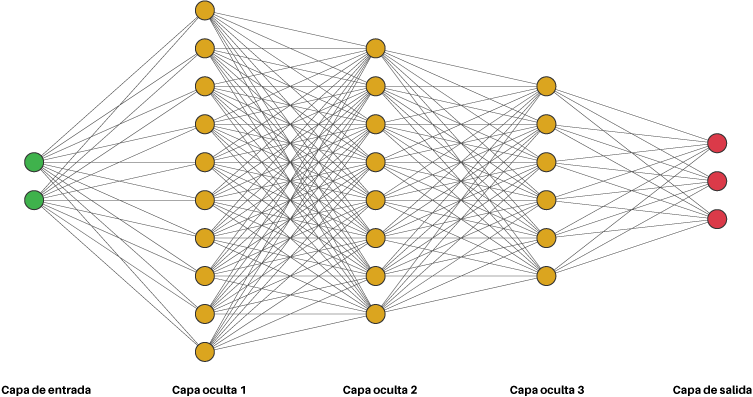
\includegraphics[width=0.6\textwidth]{imagenes_doc/redes_neuronales.png}
  \caption{Estructura de una red neuronal profunda.}
  \label{fig:logo}
\end{figure}



\subsection{Tipos Comunes de redes neuronales artificiales}

Las redes neuronales prealimentadas (FF) son una de las formas más antiguas de redes neuronales, ya que los datos fluyen en una dirección a través de capas de neuronas artificiales hasta que se obtiene el resultado. En la actualidad, la mayoría de las redes neuronales prealimentadas se consideran “prealimentadas profundas”, con varias capas (y más de una capa oculta). Las redes neuronales prealimentadas suelen vincularse a un algoritmo de corrección de errores llamado “propagación inversa” que, en términos simples, comienza con el resultado de la red neuronal y realiza el proceso en sentido inverso para llegar al principio, detectando errores para mejorar la exactitud de la red neuronal [12].

Las redes neuronales recurrentes (RNN) difieren de las redes neuronales prealimentadas en que suelen usar datos de series temporales o datos que involucran secuencias. A diferencia de las redes neuronales prealimentadas, que usan ponderaciones en cada nodo de la red, las redes neuronales recurrentes tienen memoria de lo que sucedió en la capa anterior como contingente a la salida de la capa actual. Por ejemplo, cuando se realiza procesamiento de lenguaje natural, las RNN pueden tener en cuenta otras palabras usadas en una oración. Las RNN a menudo se usan para el reconocimiento de voz, la traducción y la generación de descripciones de imágenes [12].

Este tipo de redes neuronales en las que los datos entran por la capa de entrada y se transmiten en una única dirección hacia la capa de salida -sin formar bucles, por ejemplo- son las que hemos llamado Redes Neuronales Prealimentadas o Feedforward Neural Networks en inglés. Un ejemplo de este tipo de redes:

\begin{figure}[H]
  \centering
  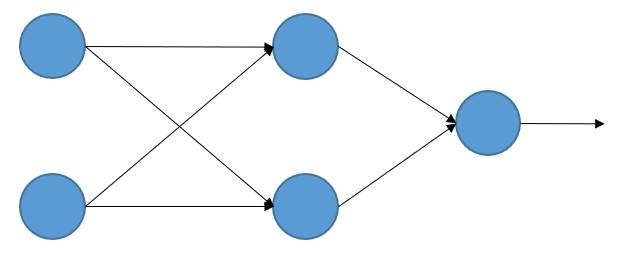
\includegraphics[width=0.6\textwidth]{imagenes_doc/image_01.jpg}
  \caption{La imagen representa una red neuronal prealimentada, uno de los modelos más básicos y utilizados en inteligencia artificial.}
  \label{fig:logo}
\end{figure}

Sin embargo, compárese esta arquitectura con la siguiente:

\begin{figure}[H]
  \centering
  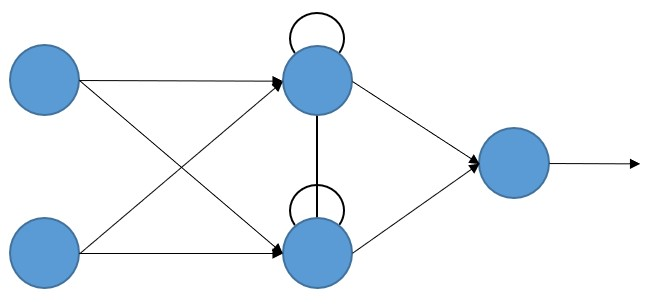
\includegraphics[width=0.6\textwidth]{imagenes_doc/image_02.jpg}
  \caption{Representación de una red neuronal recurrente (RNN), donde las conexiones internas permiten el manejo de secuencias mediante memoria temporal.}
  \label{fig:logo}
\end{figure}

La memoria a largo/corto plazo (LSTM) es una forma avanzada de RNN que puede usar memoria para recordar lo que sucedió en capas anteriores. La diferencia entre las RNN y las LSTM es que estas últimas pueden recordar lo que sucedió hace varias capas mediante el uso de celdas de memoria. La LSTM suele usarse para el reconocimiento de voz y la realización de predicciones.

Las redes neuronales convolucionales (CNN) incluyen algunas de las redes neuronales más comunes en la inteligencia artificial moderna. Las CNN suelen usarse en el reconocimiento de imágenes y emplean varias capas distintas (una capa convolucional y, luego, una capa de agrupación) que filtran diferentes partes de una imagen antes de volver a unirla (en la capa completamente conectada).
\begin{figure}[H]
  \centering
  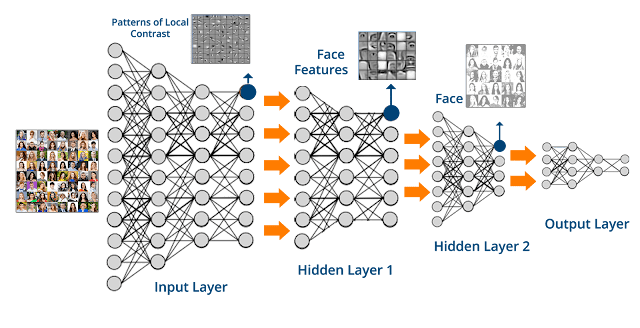
\includegraphics[width=0.6\textwidth]{imagenes_doc/redes_convolucionales.png}
  \caption{La imagen muestra cómo una red neuronal convolucional (CNN) procesa una imagen en distintas capas, extrayendo características progresivas desde patrones simples hasta rostros completos para generar una salida final.}
  \label{fig:logo}
\end{figure}

En las redes generativas adversarias (GAN), se usan dos redes neuronales que compiten entre sí en un juego que, en última instancia, mejora la exactitud del resultado. Una red (el generador) crea ejemplos que la otra red (el discriminante) juzga como verdaderos o falsos. Las GAN se han usado para crear imágenes realistas y hasta hacer arte [12].

\begin{figure}[H]
  \centering
  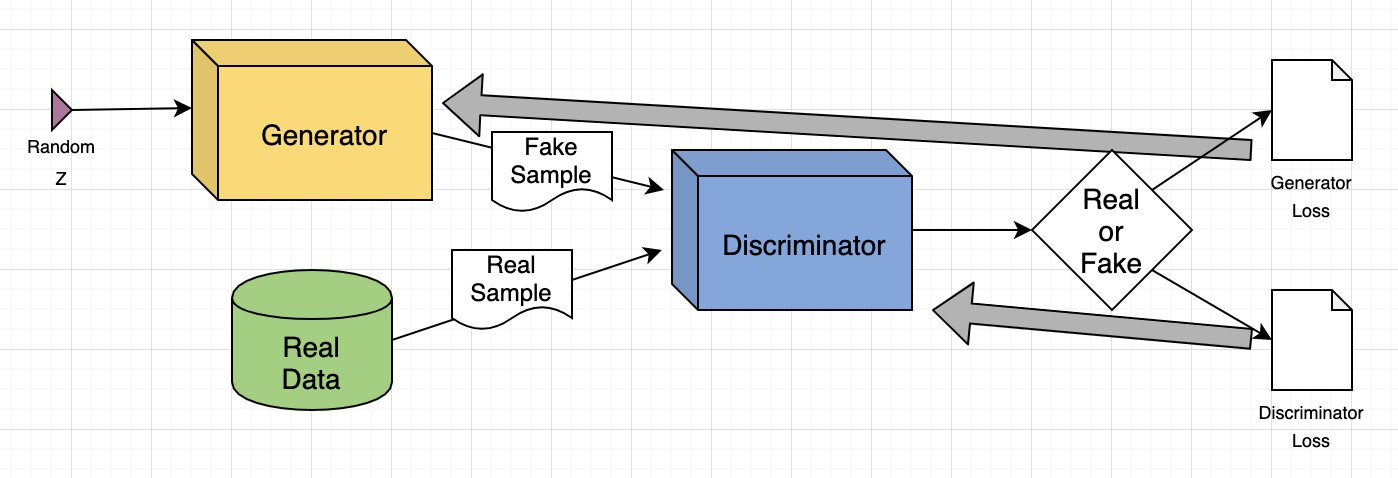
\includegraphics[width=0.6\textwidth]{imagenes_doc/Redes_GAN.jpg}
  \caption{La imagen ilustra el funcionamiento de una red generativa adversaria (GAN), donde un generador crea muestras falsas a partir de ruido aleatorio y un discriminador intenta distinguir entre muestras reales y falsas, retroalimentando a ambos modelos para mejorar su rendimiento.}
  \label{fig:logo}
\end{figure}



\subsection{Concepto de Registros Académicos.}
Los registros académicos son la recopilación sistemática de información relacionada con el desempeño, progreso y trayectoria académica de un estudiante. Esta información se almacena en diversos formatos (digitales o físicos) y es administrada por instituciones educativas, como escuelas, colegios, universidades, etc. [12].
\begin{figure}[H]
  \centering
  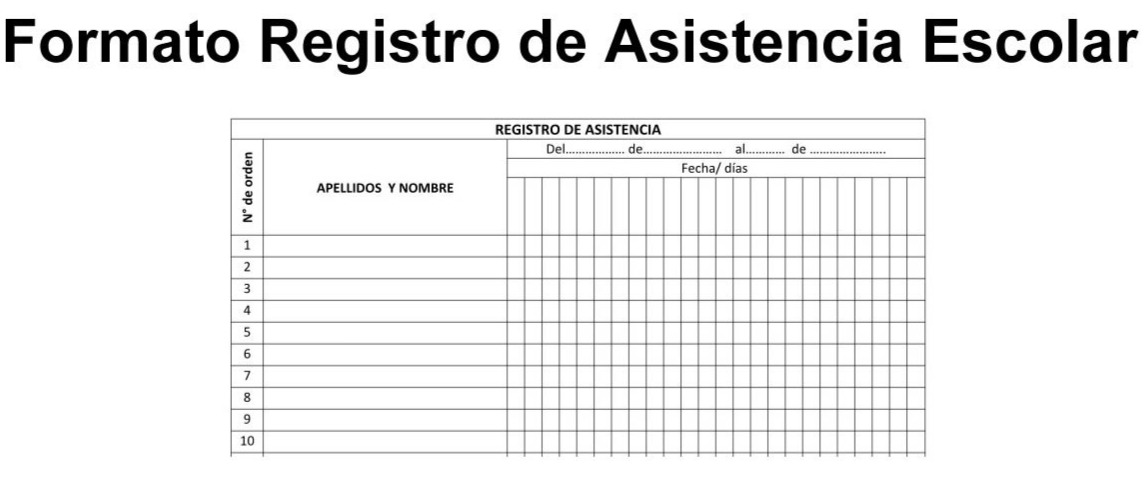
\includegraphics[width=0.6\textwidth]{imagenes_doc/registroimg.jpg}
  \caption{La imagen muestra un formato tradicional de registro de asistencia escolar, utilizado por docentes para anotar la presencia diaria de los alumnos a lo largo de un período determinado.}
  \label{fig:logo}
\end{figure}



\subsection{¿Qué contienen los registros académicos}
Los registros académicos pueden incluir:

\begin{itemize}
  \item \textbf{Calificaciones:} Notas obtenidas en cada asignatura y evaluaciones.
  \item \textbf{Asistencia:} Registro de las clases a las que el estudiante ha asistido.
  \item \textbf{Cursos aprobados:} Lista de materias completadas con éxito.
  \item \textbf{Actividades Extracurriculares:} Participación en clubes, deportes, proyectos, etc.
  \item \textbf{Información Personal:} Nombre completo, fecha de nacimiento, dirección, etc.
  \item \textbf{Historial académico:} Transferencias a otras instituciones, cambios de carrera, etc.
\end{itemize}


\subsection{¿Para qué sirven los registros académicos?}
Los registros académicos cumplen diversas funciones importantes:
\begin{itemize}
  \item \textbf{Evaluación del desempeño:} Permiten evaluar el progreso académico a lo largo del tiempo.
  \item \textbf{Toma de decisiones:} Sirven de base para tomar decisiones importantes, como la promoción a un nuevo grado, la obtención de títulos o la admisión a programas de estudios superiores.
  \item \textbf{Seguimiento académico:} Facilitan el seguimiento del progreso del estudiante y la identificación de áreas en las que necesita apoyo adicional.
  \item \textbf{Información para terceros:} Se utilizan para proporcionar información a terceros, como universidades, empleadores y agencias gubernamentales.
\end{itemize}

\subsection{Importancia de los registros académicos.}
Los registros académicos son fundamentales para garantizar la transparencia, la equidad y la calidad en el proceso educativo. Además, proporcionan un historial completo del desempeño académico de un estudiante, lo que es de gran utilidad para su futuro personal y profesional [12].


\section{Antecedentes}

\subsection{``\textit{Detección facial mediante OpenCV.}''}

El trabajo Detección facial mediante OpenCV [13], desarrollado como TFG en la FPUNE, se centra en el diseño e implementación de un software de detección facial como primer paso en el proceso de reconocimiento de rostros. En este proyecto, se realizó un exhaustivo análisis de los sistemas y técnicas de reconocimiento facial más avanzados en el estado del arte, seleccionando aquellos más relevantes para los objetivos del estudio. Proporciona una descripción detallada de las distintas etapas del proceso y su implementación, utilizando la biblioteca OpenCV y la plataforma Java. La principal contribución de este trabajo al proyecto propuesto es el método de detección facial en tiempo real y fuera de línea desde archivos.


\subsection{``\textit{Sistema de examen en línea con reconocimiento facial.}''}

El trabajo Sistema de examen en línea con reconocimiento facial [14], desarrollado como parte de un proyecto, se centra en el diseño y desarrollo de un sistema web de detección facial para mitigar intentos de fraude en evaluaciones en línea. Utilizando herramientas de código abierto como OpenCV y la plataforma Java, el sistema verifica la identidad del alumno al inicio y durante toda la evaluación, detectando tanto la ausencia del estudiante como la presencia de más de una persona. Este sistema fue probado y evaluado, mostrando resultados favorables en términos de satisfacción de los usuarios.


\subsection{``\textit{Sistema biométrico de reconocimiento facial utilizando redes neuronales artificiales en Raspberry Pi.}''}

El trabajo Sistema biométrico de reconocimiento facial utilizando redes neuronales artificiales en Raspberry Pi [15], desarrollado en una Raspberry Pi 3, se centra en el diseño e implementación de un sistema biométrico de reconocimiento facial. El sistema emplea una cámara para capturar el rostro y utiliza técnicas de inteligencia artificial y visión por computador para identificar a las personas. Para la detección de rostros, se aplica un clasificador tipo cascada, mientras que las redes neuronales convolucionales (RNC) se utilizan para el entrenamiento y reconocimiento de las imágenes faciales. El objetivo principal de este trabajo es reducir el tiempo de identificación y mejorar la precisión en entornos diversos.

\subsection{``\textit{Prototipo de reconocimiento facial para mejorar el control de asistencia de estudiantes en UNIANDES, Quevedo.}''}

El trabajo Prototipo de reconocimiento facial para mejorar el control de asistencia en UNIANDES – Quevedo [16] tiene como objetivo diseñar un prototipo de reconocimiento facial para optimizar el control de asistencia de estudiantes y la identificación facial en el laboratorio de cómputo. Este prototipo automatizó el proceso de registro de asistencia de docentes y estudiantes mediante el reconocimiento facial, facilitando la tarea con rapidez y exactitud. El sistema funciona colocando al docente frente a la cámara instalada en la parte exterior del laboratorio, activando por reconocimiento facial el dispositivo que abre la puerta, enciende el aire acondicionado y las luces. Posteriormente, los estudiantes se colocan uno por uno frente a la cámara, que detecta sus rostros y los compara con los datos almacenados en la base de datos.

\subsection{``\textit{Registro de asistencia de alumnos por medio de reconocimiento facial utilizando visión artificial}''}

El trabajo Sistema de control de asistencia para alumnos utilizando reconocimiento facial [17] se centra en el desarrollo de un sistema que emplea reconocimiento facial para registrar la asistencia de estudiantes. Implementado con redes neuronales artificiales como HOG y CNN en una Raspberry Pi 3, este proyecto busca ofrecer una solución eficiente y en tiempo real. Utilizando tecnología de visión artificial, el sistema captura y compara imágenes faciales, proporcionando un control preciso de asistencia. Diseñado para instituciones educativas, este sistema destaca por ser robusto, flexible y por optimizar la gestión de estudiantes, mejorando la eficiencia en el registro de asistencia.

\subsection{``\textit{Reconocimiento facial para la automatización del registro de asistencia a clases}''}


El trabajo Sistema piloto de registro automático de asistencia a clases presenciales FRARCA [18] se desarrolló como un sistema basado en técnicas de detección y reconocimiento facial mediante modelos de aprendizaje profundo. Diseñado con una arquitectura modular, integra herramientas como contenedores y el lenguaje de programación Python, junto con los frameworks FastAPI y Django, además de frameworks de Machine Learning como Keras, TensorFlow, PyTorch, OpenCV y MXNet. El proceso de identificación se realiza mediante la extracción y almacenamiento de características faciales en bases de datos, comparando similitudes entre vectores de características (embeddings). Esto permite eliminar la necesidad de reentrenar las redes neuronales convolucionales con cada nuevo alumno, optimizando la eficiencia del sistema.




















